\title{Game of Life Description}


\documentclass[]{article}
    
    \usepackage{graphicx}
    \usepackage{float}
\usepackage{caption}
    \usepackage{subfigure}
\begin{document}
\maketitle
\section{Question 1: Program for the Game Of Life}

Imagine every point in a grid is a life. For a point \textit{A} in the grid, 
there are 8 points around it. If there is a blackpoint, it means 
that the point is alive (otherwise it's dead). If 3 of the 8 points are alive, then the 
number of point 
\textit{A} is 3 ( "3" represents the number of living points within 8 surrounding nodes).\\

\noindent{For example, Figure 1(a) is a grid with four rows and four columns.
The corresponding number grid for Figure 1(a) is Figure 1(b).}\\

\begin{figure} 
    \centering 
    \subfigure[status for living and dead nodes]{ 
      %\label{fig:subfig:a} %% label for first subfigure 
      
\includegraphics[width=1.1in]{001.png} 
      \label{fig:label1}
    } 
    \subfigure[living number of current status]{ 
      %\label{fig:subfig:b} %% label for second subfigure 
      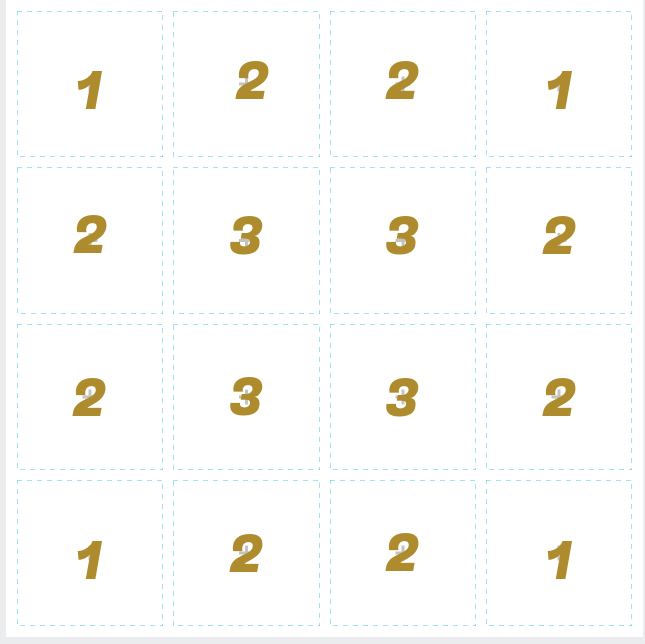
\includegraphics[width=1.1in]{002.png} 
      \label{fig:label2}
    }
        \caption{Living number for every point in a grid} 
    \label{fig::label10}
    %\label{fig:subfig} %% label for entire figure 
\end{figure}

\noindent{The living nodes in a grid changes generation by generation according to 
the number of neighbors that are \textbf{alive}, as follows:}

\begin{itemize}

    \item[1.] The neighbor of a given node are the eight nodes that touch it vertically, horizontally, or diagonally.
    \item[2.] If a node is alive but either has no neighboring nodes alive or only one alive, then in the next generation the node dies of loneliness.
    \item[3.] If a node is alive and has four or more neighboring nodes also alive, then in the next generation the node dies of overcrowding.
    \item[4.] A living node with \textbf{either two or three} living neighbors remains alive in the next generation.
    \item[5.] If a node is dead, then in the next generation it will become alive if it has \textbf{exactly three} neighboring nodes, no more, no fewer, that are already alive. All other dead nodes remain dead in the next generation.
    \item[6.] All births and deaths take place at exactly the same time, so that dying nodes can help to give birth to another, but cannot prevent the death of others by reducing overcrowding; nor can nodes being born either preserve or kill nodes living in the previous generation.     
    
\end{itemize}

\noindent{An example is shown in Figure \ref{fig:label6}. Your goal is to write a python 
program that will show how an initial configuration will change from generation to generation.}\\

\begin{figure} 
    \centering 
    \subfigure[initial status]{ 
      %\label{fig:subfig:a} %% label for first subfigure 
      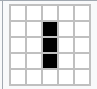
\includegraphics[width=1.1in]{003.png} 
      \label{fig:label3}
    } 
    \subfigure[first generation]{ 
      %\label{fig:subfig:b} %% label for second subfigure 
      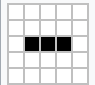
\includegraphics[width=1.1in]{004.png} 
      \label{fig:label4}
    } 
    \subfigure[second generation]{ 
      %\label{fig:subfig:b} %% label for second subfigure 
      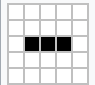
\includegraphics[width=1.1in]{004.png} 
      \label{fig:label5}
    } 
    \caption{Changes of generation} 
    \label{fig:label6}
    %\label{fig:subfig} %% label for entire figure 
\end{figure}

\noindent\textbf{Important------Sample input and Output}\\


\noindent{Your program should take input as:}\\

\noindent5\\
3\\
5\\
0\\
2\\
1\\
2\\
2\\
2\\

\noindent{The explanation for these input is:}\\

\noindent5  ---  it's a 5*5 grid (the grid size)\\
3  ---  initial living node number (how much living node in an initial status)\\
5  ---  generation number (how many generations have gone through)\\
0  ---  The abscissa of the first living point\\
2  ---  The ordinate of the first living point\\
1  ---  The abscissa of the second living point\\
2  ---  The ordinate of the second living point\\
2  ---  The abscissa of the third living point\\
2  ---  The ordinate of the third living point\\


\noindent{For the output, you have to output {1} if it's a living node, or {0}
if it's dead. Your program should output \textbf{every line} of final generation as a \textbf{list}.
For the above example, the list for the final generation should be:}\\

[[0, 0, 0, 0, 0], [0, 1, 1, 1, 0], [0, 0, 0, 0, 0], [0, 0, 0, 0, 0], [0, 0, 0, 0, 0]]\\

\noindent\textbf{The output is a list, elements are lists as well!}\\

\noindent{To make sure you have understood the rule, another running process is shown in below }

\begin{figure}[H]
    \centering 
    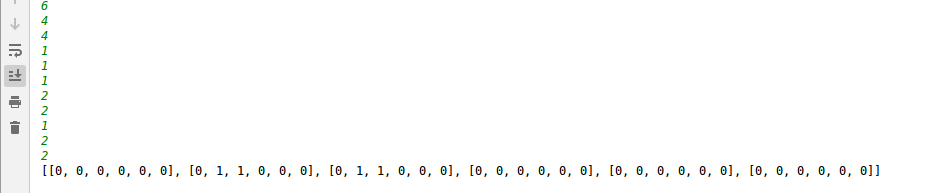
\includegraphics[width=6.7in]{oc.png} 
    \label{fig:label1}
\end{figure}

\noindent\textbf{Hint}\\

In order to put a list as an element into another list, you can use \textit{list.append()} function.
\end{document}
